\documentclass[t]{beamer}
\usepackage{mathtools}
\usepackage{tikz}
\usepackage{pgfplots}
\usepackage{ulem}
\usetikzlibrary{arrows,backgrounds,shapes,matrix,positioning,fit}
\newcommand{\argmax}{\operatornamewithlimits{argmax}}
\newcommand{\argmin}{\operatornamewithlimits{argmin}}
\newcommand{\wt}{\operatornamewithlimits{wt}}
\renewcommand\Re{\operatorname{Re}}
\renewcommand\Im{\operatorname{Im}}

\mode<presentation>
{
  \usetheme{Singapore}
  %\useoutertheme{infolines} % Showing only current section in navigation
  \setbeamertemplate{headline}{}  % Empty headline
  \setbeamertemplate{footline}[frame number]  % Getting rid of footer items except slide number
  \setbeamercovered{invisible}
  \beamertemplatenavigationsymbolsempty % Getting rid of navigation bullets at the bottom
}
\usepackage[english]{babel}
\usepackage[latin1]{inputenc}
\usepackage{times}
\usepackage[T1]{fontenc}

\title[EE 703 DMT]{Digital Modulation}
\author[Saravanan V]
{
  Saravanan Vijayakumaran\\
  \href{mailto:sarva@ee.iitb.ac.in}{sarva@ee.iitb.ac.in}
}
\institute[IIT Bombay]
{
  Department of Electrical Engineering\\
  Indian Institute of Technology Bombay
}
\date{August 19, 2013}

\AtBeginSection[]%
{%
\begin{frame}[plain]%
  \topskip0pt
  \vspace*{\fill}
    \begin{center}%
      \usebeamerfont{section title}\insertsection%
    \end{center}%
  \vspace*{\fill}
\end{frame}%
}

\begin{document}

\begin{frame}
  \titlepage
\end{frame}

%% Frame %%
\begin{frame}{Digital Modulation}
  \footnotesize
  \pause
  \begin{definition}
    The process of mapping a bit sequence to signals for transmission over a channel.
  \end{definition}
  \pause
  \begin{figure}
  \centering
  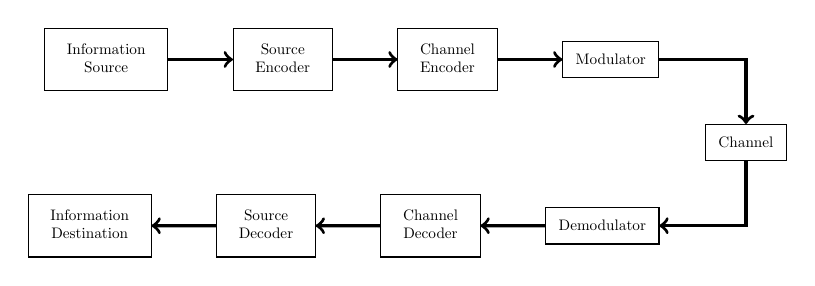
\begin{tikzpicture}[scale=0.55,transform shape]
  \tikzstyle{rectblock}=[rectangle, draw, inner sep=3mm]
  \node[rectblock] (Source) {\begin{tabular}{c} Information\\
                                                Source
                             \end{tabular}};
  \node[rectblock, right=1.5cm of Source] (Source Encoder) {\begin{tabular}{c}Source\\
                                                                             Encoder
                                                           \end{tabular}};
  \node[rectblock, right=1.5cm of Source Encoder] (Channel Encoder) {\begin{tabular}{c}Channel\\
                                                                             Encoder
                                                           \end{tabular}};
  \node[rectblock, right=1.5cm of Channel Encoder] (Modulator) {Modulator};
  \node[rectblock, below right=1.5cm of Modulator] (Channel) {Channel};
  \node[rectblock, below left=1.5cm of Channel] (Demodulator) {Demodulator};
  \node[rectblock, left=1.5cm of Demodulator] (Channel Decoder) {\begin{tabular}{c}Channel\\
                                                                               Decoder
                                                             \end{tabular}};
  \node[rectblock, left=1.5cm of Channel Decoder] (Source Decoder) {\begin{tabular}{c}Source\\
                                                                               Decoder
                                                             \end{tabular}};
  \node[rectblock, left=1.5cm of Source Decoder] (Destination) {\begin{tabular}{c} Information\\
                                                                                   Destination
                                                                \end{tabular}};
  \draw [->,very thick] (Source) -- (Source Encoder);
  \draw [->,very thick] (Source Encoder) -- (Channel Encoder);
  \draw [->,very thick] (Channel Encoder) -- (Modulator);
  \draw [->,very thick] (Modulator) -| (Channel);
  \draw [->,very thick] (Channel) |- (Demodulator);
  \draw [->,very thick] (Demodulator) -- (Channel Decoder);
  \draw [->,very thick] (Channel Decoder) -- (Source Decoder);
  \draw [->,very thick] (Source Decoder) -- (Destination);
  \tikzset{dotted/.style={draw=black!50!white, line width=1pt,
                         dash pattern=on 1pt off 1pt,
                         inner sep=4mm, rectangle, rounded corners}};
  \end{tikzpicture}
  \label{fig:commsys}
  \end{figure}
  \normalsize
\end{frame}

%% Frame %%
\begin{frame}{Digital Modulation}
  \footnotesize
  \begin{example}[Binary Baseband PAM]
  $1 \rightarrow p(t)$ and $0 \rightarrow -p(t)$
    \begin{columns}
      \begin{column}{0.5\textwidth}
      \begin{figure}
        \centering
          \begin{tikzpicture}[scale=0.6,transform shape]
            \begin{axis}[
                         title=$p(t)$,
                         xmax=2,
                         xmin=-0.5,
                         ymax=1.5,
                         ymin=-1.5,
                         axis lines = middle,
                         ytick={1,0},
                         xtick = {0,2},
                         xticklabels = {$0$,$t$},
                         yticklabels = {$A$,0},
                        ]
              \addplot[color=blue,very thick] coordinates {(0,0) (0,1) (1,1) (1,0) };
            \end{axis}
          \end{tikzpicture}
      \end{figure}
    \end{column}

    \begin{column}{0.5\textwidth}
      \begin{figure}
        \centering
          \begin{tikzpicture}[scale=0.6,transform shape]
            \begin{axis}[
                         title=$-p(t)$,
                         xmax=2,
                         xmin=-0.5,
                         ymax=1.5,
                         ymin=-1.5,
                         axis lines = middle,
                         ytick={-1,0},
                         xtick = {0,2},
                         xticklabels = {$0$,$t$},
                         yticklabels = {$-A$,0},
                        ]
              \addplot[color=blue,very thick] coordinates {(0,0) (0,-1) (1,-1) (1,0)};
            \end{axis}
          \end{tikzpicture}
      \end{figure}
      \end{column}
    \end{columns}
    
  \end{example}
  \normalsize
\end{frame}

%% Frame %%
\begin{frame}{Classification of Modulation Schemes}
  \footnotesize
  \pause
  \begin{itemize}
    \item Memoryless 
      \begin{itemize}
        \footnotesize
        \pause
        \item Divide bit sequence into $k$-bit blocks
        \pause
        \item Map each block to a signal $s_m(t), \ \ 1 \leq m \leq 2^k$
        \pause
        \item Mapping depends only on current $k$-bit block
      \end{itemize}
    \pause
    \item Having Memory 
      \begin{itemize}
        \footnotesize
        \pause
        \item Mapping depends on current $k$-bit block and $L-1$ previous blocks
        \pause
        \item $L$ is called the constraint length
      \end{itemize}
    \pause
    \item Linear 
      \begin{itemize}
        \footnotesize
        \pause
        \item Complex baseband representation of transmitted signal has the form
          \begin{equation*}
            u(t) = \sum_{n} b_n g(t-nT)
          \end{equation*}
          where $b_n$'s are the transmitted symbols and $g$ is a fixed baseband waveform
      \end{itemize}
    \pause
    \item Nonlinear 
  \end{itemize}
  \normalsize
\end{frame}

\section{Signal Space Representation}
%% Frame %%
\begin{frame}{Signal Space Representation of Waveforms}
  \footnotesize
  \begin{itemize}
    \item \pause Given $M$ finite energy waveforms, construct an orthonormal basis
      \begin{equation*}
        s_1(t),\ldots,s_M(t) \rightarrow \underbrace{\phi_1(t),\ldots,\phi_N(t)}_{\text{Orthonormal basis}}
      \end{equation*}
      \pause
      \begin{equation*}
        \langle \phi_i, \phi_j \rangle = \pause \int_{-\infty}^{\infty} \phi_i(t) \phi_j^*(t) \ dt \pause = \left\{ \begin{tabular}{ll}
                                                                                                                      1 & \text{if $i = j$} \\
                                                                                                                      0 & \text{otherwise}
                                                                                                                    \end{tabular}
                                                                                                            \right.
      \end{equation*}
    \item \pause Each $s_i(t)$ is a linear combination of the basis vectors
      \begin{equation*}
        s_i(t) = \sum_{n=1}^{N} s_{i,n} \phi_n(t), \ \ \ \ \ i=1,\ldots,M
      \end{equation*}
    \item \pause $s_i(t)$ is represented by the vector $\mathbf{s}_i = \begin{bmatrix} s_{i,1} & \cdots & s_{i,N}  \end{bmatrix}^T$
    \item \pause The set $\{\mathbf{s}_i: 1 \leq i \leq M\}$ is called the signal space representation \pause or constellation
  \end{itemize}
  \normalsize
\end{frame}

%% Frame %%
\begin{frame}{Constellation Point to Waveform}
  \footnotesize
  \pause
  \begin{figure}
    \centering
      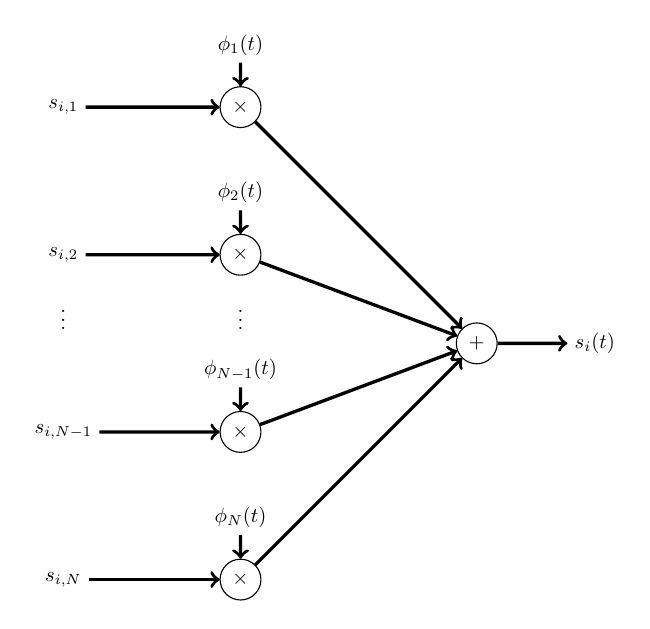
\begin{tikzpicture}[scale=0.75,transform shape]
        \tikzstyle{circblock}=[circle, draw]
        \node at (0,0) (sN) {$s_{i,N}$};
        \node at (0,2.5) (sNm1) {$s_{i,N-1}$};
        \node at (0,4.5) (vdots1) {$\vdots$};
        \node at (0,5.5) (s2) {$s_{i,2}$};
        \node at (0,8) (s1) {$s_{i,1}$};
        \node at (9,4) (st) {$s_i(t)$};
        \pause
        \node[circblock] at (3,8) (prod1) {$\times$};
        \node[circblock] at (3,5.5) (prod2) {$\times$};
        \node at (3,4.5) (vdots2) {$\vdots$};
        \node[circblock] at (3,2.5) (prodNm1) {$\times$};
        \node[circblock] at (3,0) (prodN) {$\times$};
        \draw[->,very thick] (s1) -- (prod1);
        \draw[->,very thick] (s2) -- (prod2);
        \draw[->,very thick] (sNm1) -- (prodNm1);
        \draw[->,very thick] (sN) -- (prodN);
        \pause
        \node[above=0.4 of prod1] (phi1) {$\phi_1(t)$};
        \node[above=0.4 of prod2] (phi2) {$\phi_2(t)$};
        \node[above=0.4 of prodNm1] (phiNm1) {$\phi_{N-1}(t)$};
        \node[above=0.4 of prodN] (phiN) {$\phi_N(t)$};
        \draw[->,very thick] (phi1) -- (prod1);
        \draw[->,very thick] (phi2) -- (prod2);
        \draw[->,very thick] (phiNm1) -- (prodNm1);
        \draw[->,very thick] (phiN) -- (prodN);
        \pause
        \node[circblock] at (7,4) (sum) {$+$};
        \draw[->,very thick] (prod1) -- (sum);
        \draw[->,very thick] (prod2) -- (sum);
        \draw[->,very thick] (prodNm1) -- (sum);
        \draw[->,very thick] (prodN) -- (sum);
        \draw[->,very thick] (sum) -- (st);
      \end{tikzpicture}
  \end{figure}
  \normalsize
\end{frame}

%% Frame %%
\begin{frame}{Waveform to Constellation Point}
  \footnotesize
  \pause
  \begin{figure}
    \centering
      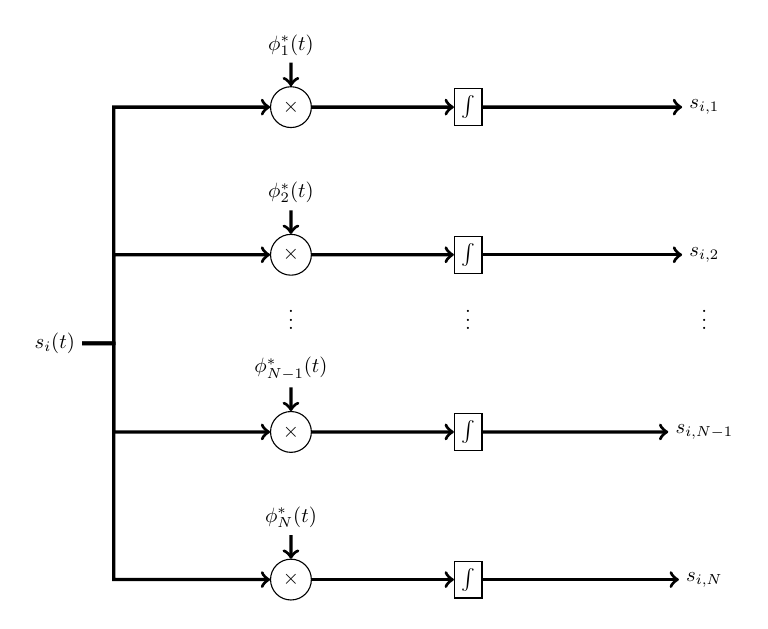
\begin{tikzpicture}[scale=0.75,transform shape]
        \tikzstyle{circblock}=[circle, draw]
        \tikzstyle{rectblock}=[rectangle, draw]
        \node at (-1,4) (st) {$s_i(t)$};
        \node at (10,0) (sN) {$s_{i,N}$};
        \node at (10,2.5) (sNm1) {$s_{i,N-1}$};
        \node at (10,4.5) (vdots1) {$\vdots$};
        \node at (10,5.5) (s2) {$s_{i,2}$};
        \node at (10,8) (s1) {$s_{i,1}$};
        \pause
        \node[circblock] at (3,8) (prod1) {$\times$};
        \node[circblock] at (3,5.5) (prod2) {$\times$};
        \node at (3,4.5) (vdots2) {$\vdots$};
        \node[circblock] at (3,2.5) (prodNm1) {$\times$};
        \node[circblock] at (3,0) (prodN) {$\times$};
        \draw[->,very thick] (st) --++(1,0) |- (prod1);
        \draw[->,very thick] (st) --++(1,0) |- (prod2);
        \draw[->,very thick] (st) --++(1,0) |- (prodNm1);
        \draw[->,very thick] (st) --++(1,0) |- (prodN);
        \pause
        \node[above=0.4 of prod1] (phi1) {$\phi_1^*(t)$};
        \node[above=0.4 of prod2] (phi2) {$\phi_2^*(t)$};
        \node[above=0.4 of prodNm1] (phiNm1) {$\phi_{N-1}^*(t)$};
        \node[above=0.4 of prodN] (phiN) {$\phi_N^*(t)$};
        \draw[->,very thick] (phi1) -- (prod1);
        \draw[->,very thick] (phi2) -- (prod2);
        \draw[->,very thick] (phiNm1) -- (prodNm1);
        \draw[->,very thick] (phiN) -- (prodN);
        \pause
        \node[rectblock] at (6,0) (intN) {$\int$};
        \node[rectblock] at (6,2.5) (intNm1) {$\int$};
        \node at (6,4.5) (vdots3) {$\vdots$};
        \node[rectblock] at (6,5.5) (int2) {$\int$};
        \node[rectblock] at (6,8) (int1) {$\int$};
        \draw[->,very thick] (int1) -- (s1);
        \draw[->,very thick] (int2) -- (s2);
        \draw[->,very thick] (intNm1) -- (sNm1);
        \draw[->,very thick] (intN) -- (sN);
        \draw[->,very thick] (prod1) -- (int1);
        \draw[->,very thick] (prod2) -- (int2);
        \draw[->,very thick] (prodNm1) -- (intNm1);
        \draw[->,very thick] (prodN) -- (intN);
      \end{tikzpicture}
  \end{figure}
  \normalsize
\end{frame}

%% Frame %%
\begin{frame}{Gram-Schmidt Orthogonalization Procedure}
  \footnotesize
  \begin{itemize}
    \item \pause Algorithm for calculating orthonormal basis for $s_1(t),\ldots,s_M(t)$
    \item \pause Consider $M = 1$
      \begin{equation*}
        \phi_1(t) = \pause \frac{s_1(t)}{\lVert s_1 \rVert}
      \end{equation*}
      where $\lVert s_1 \rVert^2 = \langle s_1, s_1 \rangle$
    \item \pause Consider $M = 2$
      \begin{eqnarray*}
        \phi_1(t) = \pause \frac{s_1(t)}{\lVert s_1 \rVert}, \ \ \  \pause \phi_2(t) = \pause \frac{\gamma(t)}{\lVert \gamma \rVert}
      \end{eqnarray*}
      \pause where $\gamma(t) = s_2(t) - \langle s_2, \phi_1 \rangle \phi_1(t)$
    \item \pause Consider $M = 3$
      \begin{eqnarray*}
        \phi_1(t) = \pause \frac{s_1(t)}{\lVert s_1 \rVert}, \ \ \ \pause
        \phi_2(t) = \pause \frac{\gamma_1(t)}{\lVert \gamma_1 \rVert}, \ \ \ \pause
        \phi_3(t) = \pause \frac{\gamma_2(t)}{\lVert \gamma_2 \rVert} \pause
      \end{eqnarray*}
      where
      \begin{eqnarray*}
        \gamma_1(t) & = & s_2(t) - \langle s_2, \phi_1 \rangle \phi_1(t) \\ \pause 
        \gamma_2(t) & = & s_3(t) - \langle s_3, \phi_1 \rangle \phi_1(t) - \langle s_3, \phi_2 \rangle \phi_2(t)
      \end{eqnarray*}
  \end{itemize}
  \normalsize
\end{frame}

%% Frame %%
\begin{frame}{Gram-Schmidt Orthogonalization Procedure}
  \footnotesize
  \begin{itemize}
    \item \pause In general, given $s_1(t),\ldots,s_M(t)$ the $k$th basis function is
      \begin{equation*}
        \phi_k(t) = \frac{\gamma_k(t)}{\lVert \gamma_k \rVert}
      \end{equation*}
    \pause where 
    \begin{equation*}
      \gamma_k(t) = s_k(t) - \sum_{i=1}^{k-1} \langle s_k, \phi_i \rangle \phi_i(t)
    \end{equation*}
    is not the zero function
    \item \pause If $\gamma_k(t)$ is zero, $s_k(t)$ is a linear combination of $\phi_1(t),\ldots,\phi_{k-1}(t)$. \pause It does not contribute to the basis.
  \end{itemize}
  \normalsize
\end{frame}

%% Frame %%
\begin{frame}{Gram-Schmidt Procedure Example}
  \footnotesize
  \begin{columns}
    \begin{column}{0.4\textwidth}
    \begin{figure}
      \centering
        \begin{tikzpicture}[scale=0.45,transform shape]
          \begin{axis}[
                       title=$s_1(t)$,
                       xmax=2.5,
                       xmin=0,
                       ymax=1.5,
                       ymin=-1.5,
                       axis lines = middle,
                       ytick={1,0},
                       xtick = {0,1,2,2.5},
                       xticklabels = {$0$,,2,$t$},
                       yticklabels = {1,0},
                      ]
            \addplot[color=blue,very thick] coordinates {(0,0) (0,1) (2,1) (2,0) };
          \end{axis}
        \end{tikzpicture}
    \end{figure}
    \begin{figure}
      \centering
        \begin{tikzpicture}[scale=0.45,transform shape]
          \begin{axis}[
                       title=$s_2(t)$,
                       xmax=2.5,
                       xmin=0,
                       ymax=1.5,
                       ymin=-1.5,
                       axis lines = middle,
                       ytick={1,-1},
                       xtick = {0,2,2.5},
                       xticklabels = {$0$,2,$t$},
                       xticklabel shift = -20pt,
                       yticklabels = {1,-1},
                      ]
            \addplot[color=blue,very thick] coordinates {(0,0) (0,1) (1,1) (1,-1) (2,-1) (2,0) };
          \end{axis}
        \end{tikzpicture}
    \end{figure}
  \end{column}

  \begin{column}{0.6\textwidth}
    \begin{figure}
      \centering
        \begin{tikzpicture}[scale=0.45,transform shape]
          \begin{axis}[
                       title=$s_3(t)$,
                       xmax=3.5,
                       xmin=0,
                       ymax=1.5,
                       ymin=-1.5,
                       axis lines = middle,
                       ytick={-1,1},
                       xtick = {0,1,3,3.5},
                       xticklabels = {$0$,,3,$t$},
                       xticklabel shift = -20pt,
                       yticklabels = {-1,1},
                       x post scale = 1.5
                      ]
            \addplot[color=blue,very thick] coordinates {(0,0) (0,1) (2,1) (2,-1) (3,-1) (3,0)};
          \end{axis}
        \end{tikzpicture}
    \end{figure}
    \begin{figure}
      \centering
        \begin{tikzpicture}[scale=0.45,transform shape]
          \begin{axis}[
                       title=$s_4(t)$,
                       xmax=3.5,
                       xmin=0,
                       ymax=1.5,
                       ymin=-1.5,
                       axis lines = middle,
                       ytick={-1,1},
                       xtick = {0,1,2,3,3.5},
                       xticklabels = {$0$,,,3,$t$},
                       xticklabel shift = -20pt,
                       yticklabels = {-1,1},
                       x post scale = 1.5
                      ]
            \addplot[color=blue,very thick] coordinates {(0,0) (0,-1) (3,-1) (3,0)};
          \end{axis}
        \end{tikzpicture}
    \end{figure}
    \end{column}
  \end{columns}
  \normalsize
\end{frame}

%% Frame %%
\begin{frame}{Gram-Schmidt Procedure Example}
  \footnotesize
  \pause
  \begin{columns}
    \begin{column}{0.4\textwidth}
    \begin{figure}
      \centering
        \begin{tikzpicture}[scale=0.45,transform shape]
          \begin{axis}[
                       title=$\phi_1(t)$,
                       xmax=2.5,
                       xmin=0,
                       ymax=1.5,
                       ymin=-1.5,
                       axis lines = middle,
                       ytick={0.707,0},
                       xtick = {0,1,2,2.5},
                       xticklabels = {$0$,,2,$t$},
                       yticklabels = {$\frac{1}{\sqrt{2}}$,0},
                      ]
            \addplot[color=blue,very thick] coordinates {(0,0) (0,0.707) (2,0.707) (2,0) };
          \end{axis}
        \end{tikzpicture}
    \end{figure}
  \pause
    \begin{figure}
      \centering
        \begin{tikzpicture}[scale=0.45,transform shape]
          \begin{axis}[
                       title=$\phi_2(t)$,
                       xmax=2.5,
                       xmin=0,
                       ymax=1.5,
                       ymin=-1.5,
                       axis lines = middle,
                       ytick={0.707,-0.707},
                       xtick = {0,2,2.5},
                       xticklabels = {$0$,2,$t$},
                       xticklabel shift = -20pt,
                       yticklabels = {$\frac{1}{\sqrt{2}}$,$-\frac{1}{\sqrt{2}}$},
                      ]
            \addplot[color=blue,very thick] coordinates {(0,0) (0,0.707) (1,0.707) (1,-0.707) (2,-0.707) (2,0) };
          \end{axis}
        \end{tikzpicture}
    \end{figure}
  \end{column}

  \pause
  \begin{column}{0.6\textwidth}
    \begin{figure}
      \centering
        \begin{tikzpicture}[scale=0.45,transform shape]
          \begin{axis}[
                       title=$\phi_3(t)$,
                       xmax=3.5,
                       xmin=0,
                       ymax=1.5,
                       ymin=-1.5,
                       axis lines = middle,
                       ytick={-1,1},
                       xtick = {0,1,2,3,3.5},
                       xticklabels = {$0$,,2,3,$t$},
                       xticklabel shift = -20pt,
                       yticklabels = {-1,1},
                       x post scale = 1.5
                      ]
            \addplot[color=blue,very thick] coordinates {(0,0) (2,0) (2,-1) (3,-1) (3,0)};
          \end{axis}
        \end{tikzpicture}
    \end{figure}
    \pause
    \begin{eqnarray*}
      \mathbf{s}_1 & = & \pause \begin{bmatrix} \sqrt{2} & 0 & 0 \end{bmatrix}^T \\
      \pause
      \mathbf{s}_2 & = & \pause \begin{bmatrix} 0 & \sqrt{2} & 0 \end{bmatrix}^T \\
      \pause
      \mathbf{s}_3 & = & \pause \begin{bmatrix} \sqrt{2} & 0 & 1 \end{bmatrix}^T \\
      \pause
      \mathbf{s}_4 & = & \pause \begin{bmatrix} -\sqrt{2} & 0 & 1 \end{bmatrix}^T 
    \end{eqnarray*}
    \end{column}
  \end{columns}
  \normalsize
\end{frame}

%% Frame %%
\begin{frame}{Properties of Signal Space Representation}
  \footnotesize
  \begin{itemize}
    \item Energy
      \begin{equation*}
        E_m = \int_{-\infty}^{\infty} \lvert s_m(t) \rvert^2 \ dt = \pause \sum_{n=1}^N \lvert s_{m,n} \rvert^2 = \pause \lVert \mathbf{s}_m \rVert^2
      \end{equation*}
    \pause
    \item Inner product
      \begin{equation*}
        \langle s_i(t), s_j(t) \rangle = \pause \langle \mathbf{s}_i,\mathbf{s}_j \rangle
      \end{equation*}
  \end{itemize}
  \normalsize
\end{frame}

\section{Modulation Schemes}

%% Frame %%
\begin{frame}{Pulse Amplitude Modulation}
  \footnotesize
  \begin{itemize}
    \item Signal Waveforms
      \begin{equation*}
        s_m(t) = A_m p(t), \ \ \ \ 1 \leq m \leq M
      \end{equation*}
      where $p(t)$ is a pulse of duration $T$ and $A_m$'s denote the $M$ possible amplitudes.
    \item \pause {\usebeamercolor[fg]{frametitle}Example} $M = 2$, $p(t)$ is a real pulse

$A_1 = -A, A_2 = A$ for a real number $A$
    \pause
    \begin{figure}
      \centering
        \begin{tikzpicture}[scale=0.7,transform shape]
          \begin{axis}[
                       xmax=4,
                       xmin=-4,
                       ymax=0.1,
                       ymin=-0.1,
                       axis lines = middle,
                       ytick=\empty,
                       xtick = data,
                       x post scale = 2.0,
                       xticklabels = {A,-A},
                       y axis line style={-},
                      ]
            \addplot+[only marks, mark options={draw=black,fill=black},] coordinates {(1,0) (-1,0)};
          \end{axis}
        \end{tikzpicture}
    \end{figure}
  \end{itemize}
  \normalsize
\end{frame}

%% Frame %%
\begin{frame}{Pulse Amplitude Modulation}
  \footnotesize
  \begin{itemize}
    \item \pause {\usebeamercolor[fg]{frametitle}Example} $M = 4$, $p(t)$ is a real pulse

$A_1 =-3A, A_2 =-A, A_3 = A, A_4 = 3A$ 
    \pause
    \begin{figure}
      \centering
        \begin{tikzpicture}[scale=0.7,transform shape]
          \begin{axis}[
                       xmax=4,
                       xmin=-4,
                       ymax=0.1,
                       ymin=-0.1,
                       axis lines = middle,
                       ytick=\empty,
                       xtick = data,
                       x post scale = 2.0,
                       xticklabels = {-3A,-A,A,3A},
                       y axis line style={-},
                      ]
            \addplot+[only marks, mark options={draw=black,fill=black},] coordinates {(-3,0) (-1,0) (1,0) (3,0)};
          \end{axis}
        \end{tikzpicture}
    \end{figure}
  \end{itemize}
  \normalsize
\end{frame}

%% Frame %%
\begin{frame}{Phase Modulation}
  \footnotesize
  \begin{itemize}
    \item Complex envelope of phase modulated signals
      \begin{equation*}
        s_m(t) = p(t)e^{\ j\frac{\pi(2m-1)}{M}}, \ \ \ \ 1 \leq m \leq M
      \end{equation*}
      where $p(t)$ is a real baseband pulse of duration $T$
    \pause
    \item Corresponding passband signals
      \begin{eqnarray*}
        s_m^p(t) & = & \Re\left[\sqrt{2}s_m(t)e^{\ j2\pi f_c t}\right] \\
                 \pause
                 & = & \sqrt{2}p(t)\cos \left(\frac{\pi(2m-1)}{M}\right) \cos 2\pi f_c t \\
                 &   & - \sqrt{2}p(t)\sin \left(\frac{\pi(2m-1)}{M}\right) \sin 2\pi f_c t 
      \end{eqnarray*}
  \end{itemize}
  \normalsize
\end{frame}

%% Frame %%
\begin{frame}{Constellation for PSK}
  \footnotesize
  \begin{figure}
    \centering
      \begin{tikzpicture}[scale=0.5,transform shape]
        \begin{axis}[
                     title={QPSK, $M=4$},
                     xmax=1.5,
                     xmin=-1.5,
                     ymax=1.5,
                     ymin=-1.5,
                     axis lines = middle,
                     ytick= \empty,
                     xtick = \empty,
                     x post scale = 1.0,
                     xticklabel shift = -20pt,
                     y axis line style={-},
                     x axis line style={-},
                     nodes near coords,
                    ]
          \addplot+[only marks, 
                    mark options={draw=black,fill=black},
                    point meta=explicit symbolic
                    ] 
                    coordinates {
                      (1,1)[11] 
                      (1,-1)[10] 
                      (-1,1)[01] 
                      (-1,-1)[00]
                    };
        \end{axis}
      \end{tikzpicture}
  \end{figure}
  \pause
  \begin{figure}
    \centering
      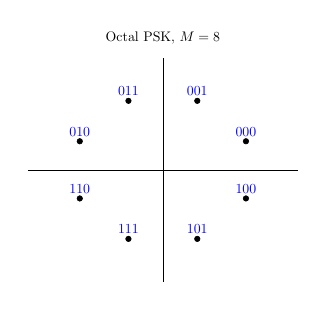
\begin{tikzpicture}[scale=0.5,transform shape]
        \begin{axis}[
                     title={Octal PSK, $M=8$},
                     xmax=1.5,
                     xmin=-1.5,
                     ymax=1.5,
                     ymin=-1.5,
                     axis lines = middle,
                     ytick= \empty,
                     xtick = \empty,
                     y axis line style={-},
                     x axis line style={-},
                     nodes near coords,
                    ]
          \addplot+[only marks, 
                    mark options={draw=black,fill=black},
                    point meta=explicit symbolic
                    ] 
                    coordinates {
                      (0.923879,0.382683432)[000] 
                      (0.382683432,0.923879)[001] 
                      (-0.382683432,0.923879)[011] 
                      (-0.923879,0.382683432)[010] 
                      (-0.923879,-0.382683432)[110] 
                      (-0.382683432,-0.923879)[111] 
                      (0.382683432,-0.923879)[101] 
                      (0.923879,-0.382683432)[100] 
                    };
        \end{axis}
      \end{tikzpicture}
  \end{figure}
  \normalsize
\end{frame}

%% Frame %%
\begin{frame}{Quadrature Amplitude Modulation}
  \footnotesize
  \begin{itemize}
    \item Complex envelope of QAM signals
      \begin{equation*}
        s_m(t) = (A_{m,i} + jA_{m,q})p(t), \ \ \ \ 1 \leq m \leq M
      \end{equation*}
      where $p(t)$ is a real baseband pulse of duration $T$
    \pause
    \item Corresponding passband signals
      \begin{eqnarray*}
        s_m^p(t) & = & \Re\left[\sqrt{2}s_m(t)e^{\ j2\pi f_c t}\right] \\
                 \pause
                 & = & \sqrt{2}A_{m,i}p(t) \cos 2\pi f_c t  - \sqrt{2}A_{m,q}p(t) \sin 2\pi f_c t 
      \end{eqnarray*}
  \end{itemize}
  \normalsize
\end{frame}

%% Frame %%
\begin{frame}{Constellation for QAM}
  \footnotesize
  \begin{figure}
    \centering
      \begin{tikzpicture}[scale=1.0,transform shape]
        \begin{axis}[
                     title={16-QAM},
                     xmax=4,
                     xmin=-4,
                     ymax=4,
                     ymin=-4,
                     axis lines = middle,
                     ytick= \empty,
                     xtick = \empty,
                     y axis line style={-},
                     x axis line style={-},
                    ]
          \addplot+[only marks, 
                    mark options={draw=black,fill=black},
                    ] 
                    coordinates {
                      (3,1)
                      (1,3)
                      (-1,3)
                      (-3,1)
                      (-3,-1)
                      (-1,-3)
                      (1,-3)
                      (3,-1)
                      (1,1)
                      (-1,1)
                      (1,-1)
                      (-1,-1)
                      (3,3)
                      (-3,3)
                      (3,-3)
                      (-3,-3)
                    };
        \end{axis}
      \end{tikzpicture}
  \end{figure}
  \normalsize
\end{frame}

%% Frame %%
\begin{frame}{}
\vfill
\begin{center}
Thanks for your attention
\end{center}
\vfill
\end{frame}

\end{document}
